\documentclass[usenatbib]{mnras}
\usepackage[T1]{fontenc}
\usepackage{ae,aecompl}

\usepackage{graphicx}	% Including figure files
\usepackage{amsmath}	% Advanced maths commands
\usepackage{amssymb}	% Extra maths symbols
\usepackage{array}

\usepackage{multirow}
\usepackage{multicol}
\usepackage{blindtext}
\newcolumntype{?}{!{\vrule width 1pt}}
\newcommand{\Msun}{\,{\rm M}$_{\odot}$\,}
\newcommand{\Mpch}{\,{\rm Mpc}\,\ifmmode h^{-1}\else $h^{-1}$\fi}
\newcommand{\kpch}{\,{\rm kpc}\,\ifmmode h^{-1}\else $h^{-1}$\fi}
\newcommand{\kpc}{\,{\rm kpc}\,}

%%%%%%%%%%%%%%%%%%% TITLE PAGE %%%%%%%%%%%%%%%%%%%
\title[Laniakea in context]{The Laniakea supercluster in a cosmological context}
\author[Barrera et al.]{
\parbox[t]{\textwidth}{
    {J. D. Pe\~naranda-Rivera $^1$,} 
    {David L.  Paipa-Le\'on$^{2}$,}
    {Sergio Hern\'andez-Charpak$^3$,}\\
    {Jaime E. Forero-Romero $^{2}$}
}
\\\\
$^{1}$ Departamento de F\'isica, Universidad de los Andes, Cra. 1
  No. 18A-10 Edificio Ip, CP 111711, Bogot\'a, Colombia \\
$^{2}$ Switzerland\\
}

% These dates will be filled out by the publisher
\date{Accepted XXX. Received YYY; in original form ZZZ}

% Enter the current year, for the copyright statements etc.
\pubyear{2019}


% Don't change these lines
\begin{document}
\label{firstpage}
\pagerange{\pageref{firstpage}--\pageref{lastpage}}
\maketitle

%%%%%====MYMARK========
\maketitle
\begin{abstract}
Galaxy superclusters can be defined as regions of converging galaxy velocity flows.
Such structures have quantifiable properties such as mass, volume and shape.
The most precise quantification of such an object has been done on our local supercluster, Laniakea. 
In this work the properties of Laniakea are compared to the expectations from a Lambda Cold Dark Matter Universe.
Cosmological N-body simulations are used in order to find cosmic flow fields of dark matter halos and find the superclusters using a watershed algorithm.
In addition, the distributions of volume, mass and shape of the superclusters found in those simulations are quantified and compared with known values for Laniakea.
In all those cases Laniakea is found in the tail of the distribution, placing it as an atypical object in a cosmological context. 
\end{abstract}

\begin{keywords}
%%PREGUNTAR
%galaxies:supercluster --- simulation:cosmological --- filter:gaussian --- methods:numerical
\end{keywords}


%=========================================================================
%		PAPER CONTENT
%=========================================================================

%*************************************************************************

\section{Introduction}
% La introduccion y el abstract es lo ultimo que se escribe.

In 2014 astronomers used a map  of peculiar velocities of galaxies to
define the Laniakea supercluster of galaxies
\citep{2014Natur.513...71T}.  
Their main input was the Cosmicflows-2 catalog of distances and radial
velocities that provide them with coverage of distances up to Mpc. 
From these data they After performing a Wiener fiter reconstruction of
3-dimensional velocities.
Then they define Laniakea as  a region within walls of divergence velocity.  
Laniakea thus represents is a region of inflowing peculiar velocities
that include the Milky Way. 

Laniakea has a very isotropic shape. 
Its radius is approximately $160$ Mpc and encompasses a mass of
$\approx 10^{17}$ \Msun.



\section{Cosmological N-body data}

We use data from the dark matter only cosmological simulations with
$720$ \Mpch on a side from the Abacus Cosmos project.  
These boxes were simulated with $1440^3$ particles in a background
cosmology following Planck 2015 parameters, although a set of
different simulations will be analyzed in order to determine the
relevance of cosmological parameters.
The resolution of these simulations correspond to a DM particle mass
of $\sim 1 \times 10^{10}$\Msun.
We use the Friend-of-Friends catalogs at redshift $z=0.1$.
The halos included in those catalogs have a lower mass bound of 
maximum circular velocity of $V_{\rm circ}=50$ \kms.
In our case we only use halos with maximum circular velocity larger
than $300$ \kms.
Changing that limit down to $200$ \kms does not significantly affect
the results we report here.

\subsection{Grid Construction}  

The simulation volume was segmented into a cubic gride of side $N_{side}=360$, 
which corresponds to a cubic cell size of $L_{cell}=2$ Mpc/h.
Following \cite{2014Natur.513...71T} the velocity of each DM halo was interpolated onto the
grid using a Cloud-In-Cell (CIC) scheme. 
This CIC grid is then convolved with a three dimensional gaussian of scale $\sigma_s$.
Different values for this scale were used in order to visualize the effects of the interpolation. However, the value of $10$ Mpc/h is close to the nominal value for the equivalent spatial resolution
in the Cosmic Flows studies that led to the delimitation of Laniakea. As a result, the value of $\sigma_s$ selected to be used in the watershed algorithm was $10$ Mpc/h. It is convenient to stlished a new variable, which will be used often in this paper, as $\sigma_{Vox}$ = $\sigma_s$/$L_{cell}$, which will represent a dimensionless gaussian smoothing scale. 
Finally, we compute the divergence of the interpolated and smoothed velocity field using a
finite difference scheme; with this choice high density regions should have low negative
values for the divergence.


\subsection{Finding superclusters}
\label{sec:INTROWatershed}

We use watershed segmentation to define the superclusters.
This methods segments a scalar field into disjoints groups \citep{BeucherWatershed1979}.
Our implementation works as follows . 
We sweep the cells in the divergence grid from the lowest values to the highest, i.e. from
the high density regions with converging flows to the lowest density regions with divergent
flows.
For the $i$-th cell under consideration we check whether its 28 neighbors have already been assigned to a group. 
If all the neighbors are unassigned, then this $i$-th cell starts a new group; if the majority of already assigned cells belongs to the $n$-th group, then this cell belongs to that group. 
At the end of the sweep all cells have been assigned to a group.
In all our calculations we take periodical boundary conditions into account. 
We highlight that this algorithms do not have free parameters based either on divergence, density or distance thresholds.
Finally, for each supercluster we compute its volume together with the eigenvalues and eigenvectors of the inertia tensor.


\section{Results}




\begin{figure}
    \centering
    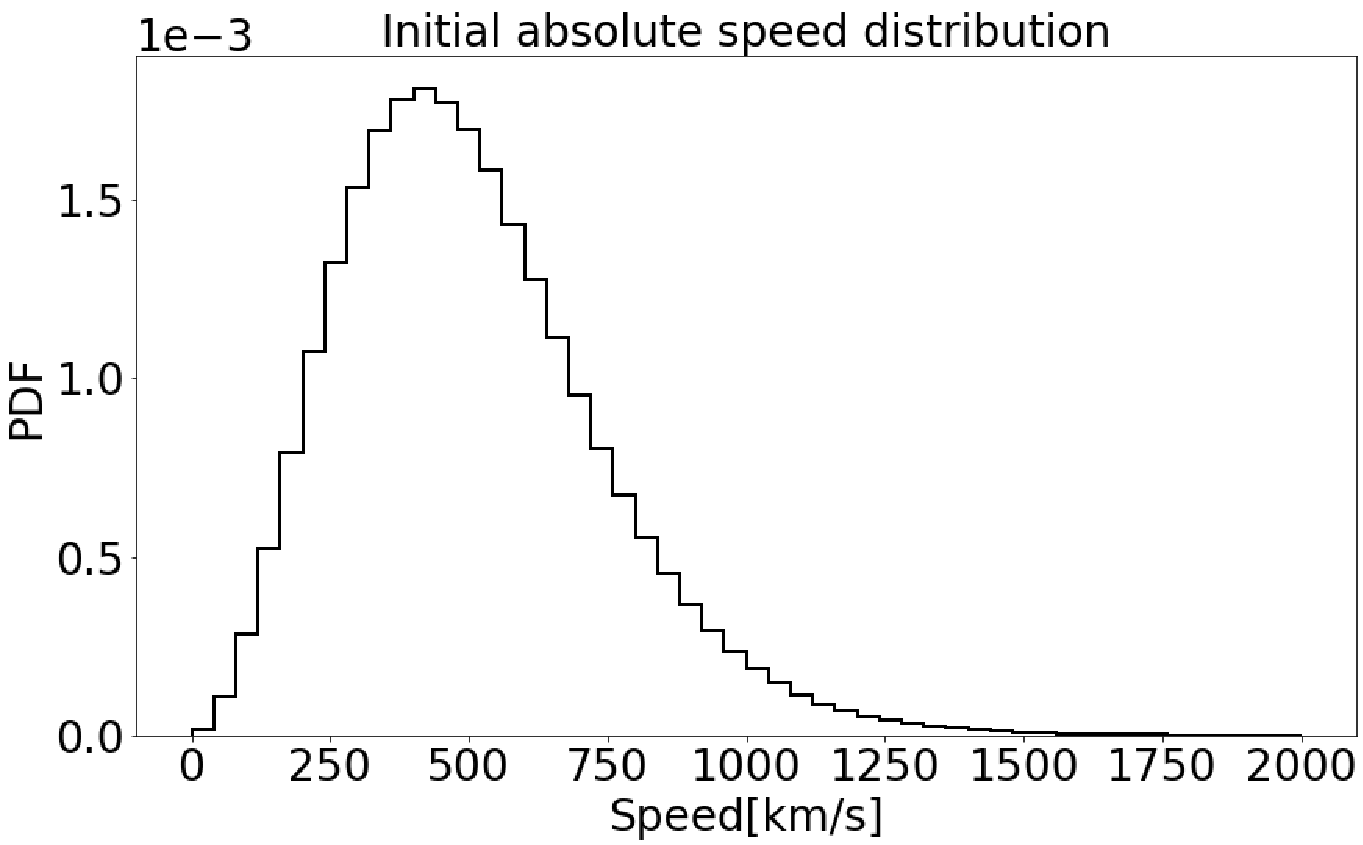
\includegraphics[width=240pt]{initial_distribution.pdf}
    \caption{Initial distribution for the speed magnitude of every mass particle, as given by the Abacus Cosmos simulation. This analysis is done without making any Gaussian filter over the speed fields.}
    \label{fig:initial_distribution}
\end{figure}


\subsection{Gaussian Convolution and Sigma relevance}

In his study about Laniakea, Tully\cite{tully_laniakea_2014} emphasizes a simple idea but with great influence on the study that will be developed. In his study is mentioned that, in cosmological frameworks, it is assumed that large-scale structure formation is due to Gaussian primordial fluctuations of the field of gravity. It is expected that as long as the density and speed fields evolution remain in the linear regime, they will keep their Gaussian properites. That is why to obtain adequate results it is necessary to take into account these Gaussian behavior of velocity and mass fields by smoothing them.

\begin{figure}
    \centering
    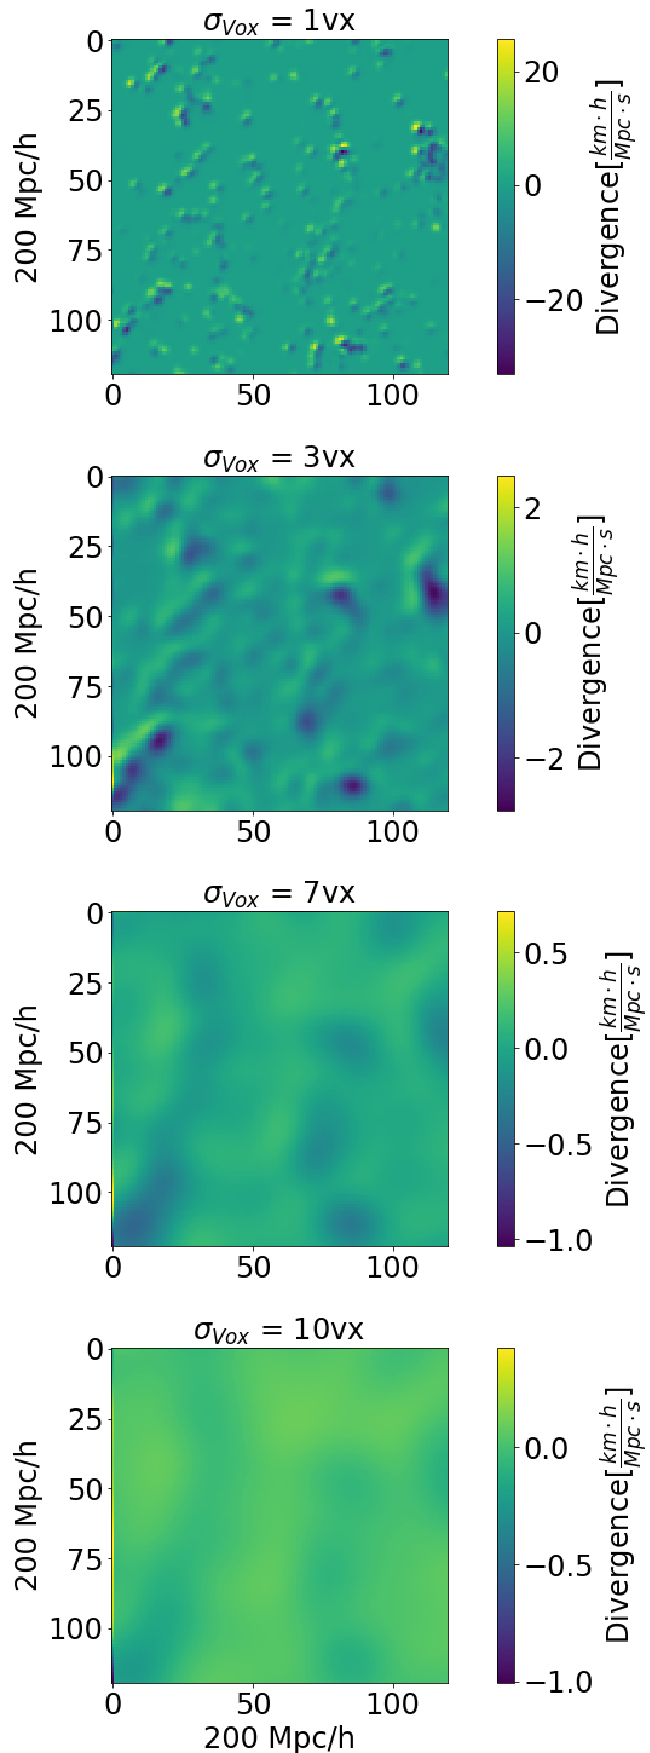
\includegraphics[height = 580pt]{grad_fields.pdf}
    \caption{Here is shown  a random cross section of the softened divergence fields. The $\sigma_{Vox}$ used for every case is shown on top of every plot. Notice how peak values decrease and defined structures start to be seen once $\sigma_{Vox}$ is increased.}
    \label{fig:SigmasVDCZcut}
\end{figure}
Also, in order to perform the watershed analysis in a divergence grid it is necesary that the scalar field represented by the grid is differentiable, otherwise the watershed algorithm will find discontinuities and eventually will lead to the misclassification of superclusters. In particular, we want velocity distribution of the grid to look such as the initial distribution of the simulation. This initial distribution is presented in figure \ref{fig:initial_distribution}.

In order to perform a complete watershed analysis over the divergence field and extend it to characterization of superclusters based on features as volume or mass,  it is necesary to apply the  \textbf{same} Gaussian Filter to the 3D axial velocity grids and the mass grid as well. This in done so that we can have consistent measures despite the smoothing of the divergence field.



\begin{figure}
    \centering
    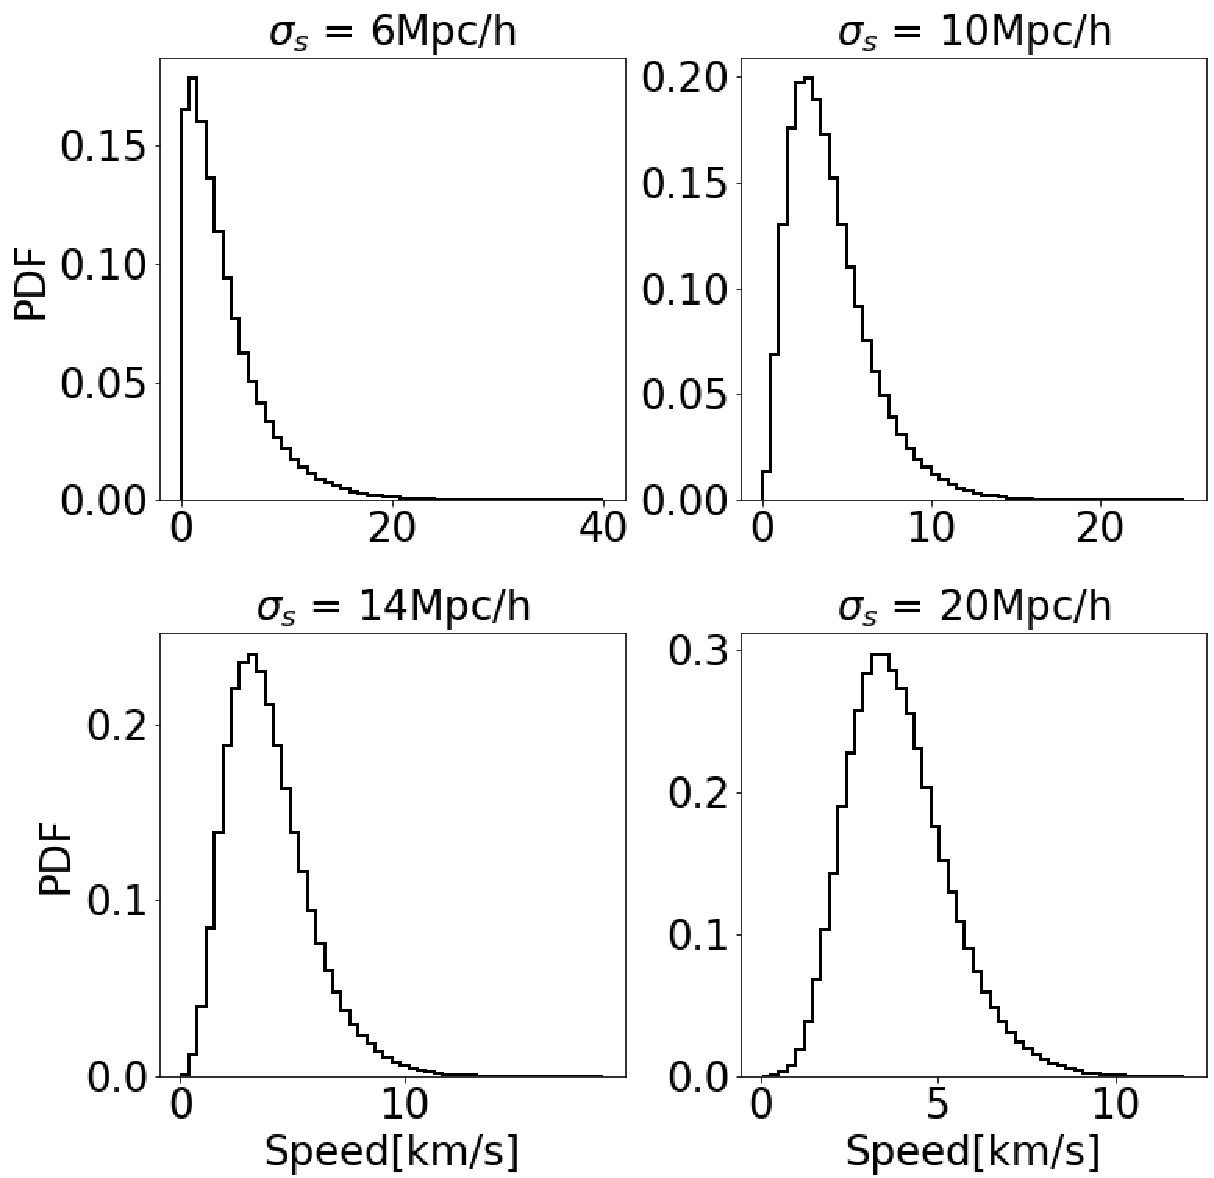
\includegraphics[width=240pt]{smooth_vel_dist.pdf}
    \caption{Distribution of the speed magnitude for the voxels in the grid calculated for different values of $\sigma_{Vox}$. Notice how the ranges of values change when $\sigma_{Vox}$ changes and the distribution becomes similar to the one seen in figure \ref{fig:initial_distribution}.}
    \label{fig:MD_Varios}
\end{figure}

To perform the smoothing, a $\sigma_{Vox}$ value is needed with aim of defining the width of the Gaussian Filter. With small $\sigma_{Vox}$\footnote{Small $\sigma$ are between 1 and 5 voxels in the grid reference. Big $\sigma$ are values of 15 voxels or more.} many structures are visible in a fine and defined network in the divergence grid, while big $\sigma_{Vox}$ only diferentiate big structures with barely any resolution of smaller filaments. Also, using big $\sigma_{Vox}$ cause peak values to be smoothed and values of the field move closer to  the average value of the field. This effects can be seen in Figure \ref{fig:SigmasVDCZcut} where the same cross-section of the divergence field grid is shown but smoothed with different values of $\sigma_{Vox}$.


\begin{figure}
    \centering
    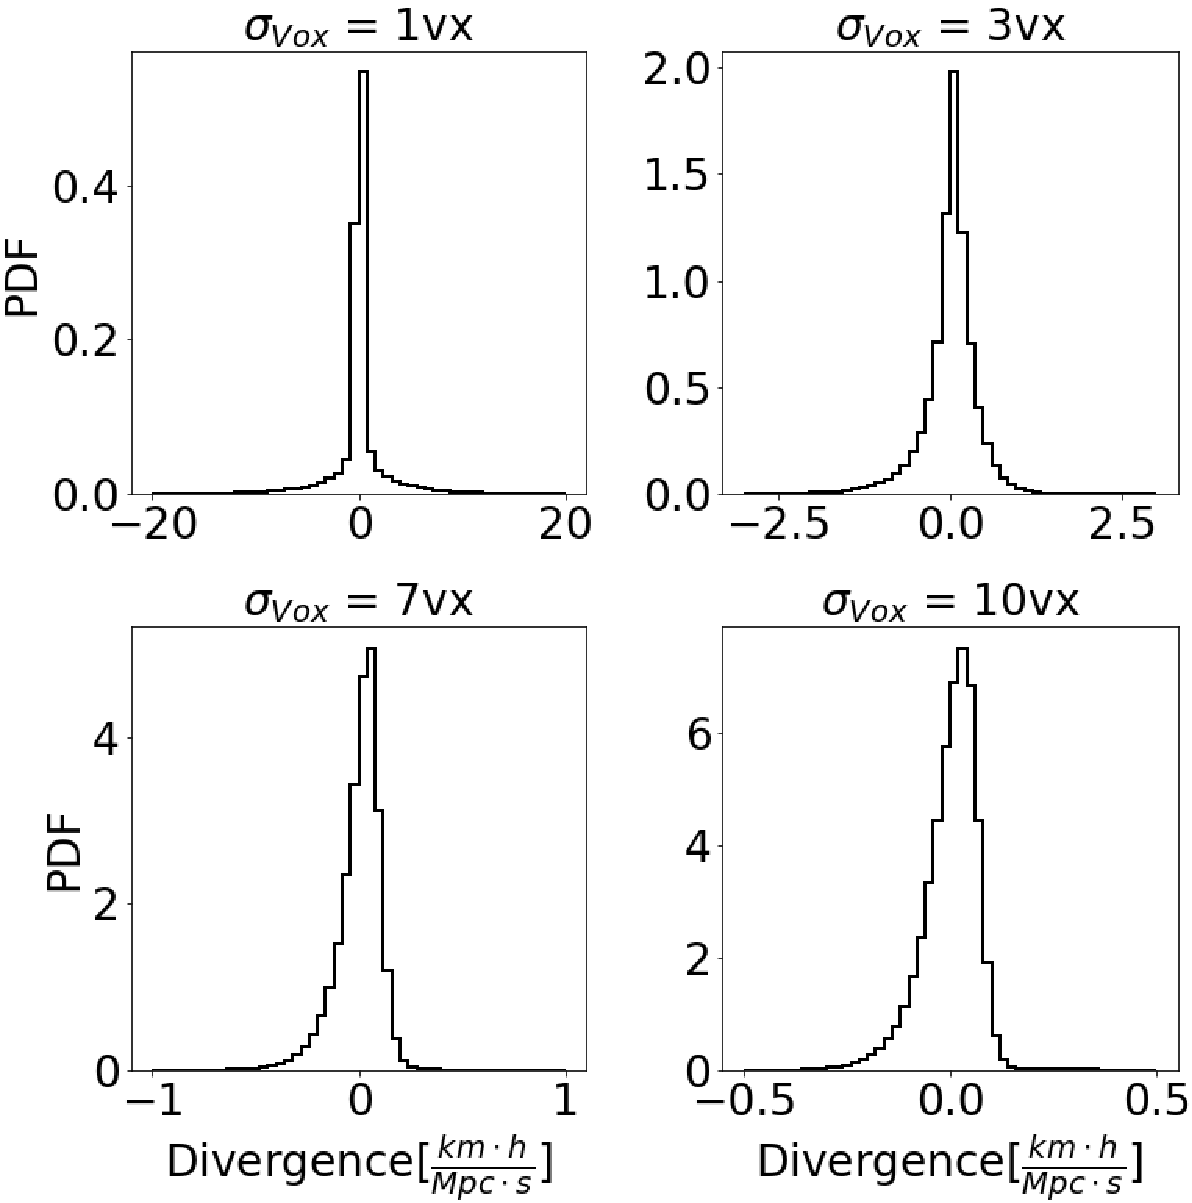
\includegraphics[width=240pt]{smooth_grad_dist.pdf}
    \caption{Distribution of the divergence field for the voxels in the grid calculated for different values of $\sigma_{Vox}$. Notice how the divergence ranges get lower when $\sigma_{Vox}$ increases.}
    \label{fig:VCD_Varios}
\end{figure}


\paragraph{Remember}  that once the $\sigma_{Vox}$ value has been chosen, the smoothing must be done for the axial velocity grids $V_x$, $V_y$, $V_z$ and the mass grid \textbf{M}. This in order to have coherent results in future processes.




Once the grids have been smoothed with a defined $\sigma_{Vox}$, it is evident that the magnitude of the values in the grids and the ones subsequently calculated is reduced. It was expected that this attenuation would happen since the interpolation brings the data closer to the field average. This can be evidenced in the figures \ref{fig:MD_Varios} and \ref{fig:VCD_Varios}.

\subsection{Interpretation of low digergence regions}
Once the Gaussian process is realized in the simulations, several regions of negative divergence are identified. These regions are interpreted as places in space where matter is coming together at high ratios. As a result, after the interpolation is executed, negative divergence regions are expected to have larger values of absolute velocities. This can be seen in Figure \ref{fig:grad_vel_fields} where the divergence field is shown in colors, where yellow zones have a big positive divergence and dark blue regions are those with big negative values for it. Notice how in these structures the divergence is much more negative in the center of the agglomerations than in the rest of the structure and how the whole structure has bigger velocity vectors than the remain regions. The last part corresponds to the structure formation process, interpreted in this context as the region where a supercluster could possibly be, and will be the first regions considered once we apply the watershed algorithm.

\begin{figure}
    \centering
    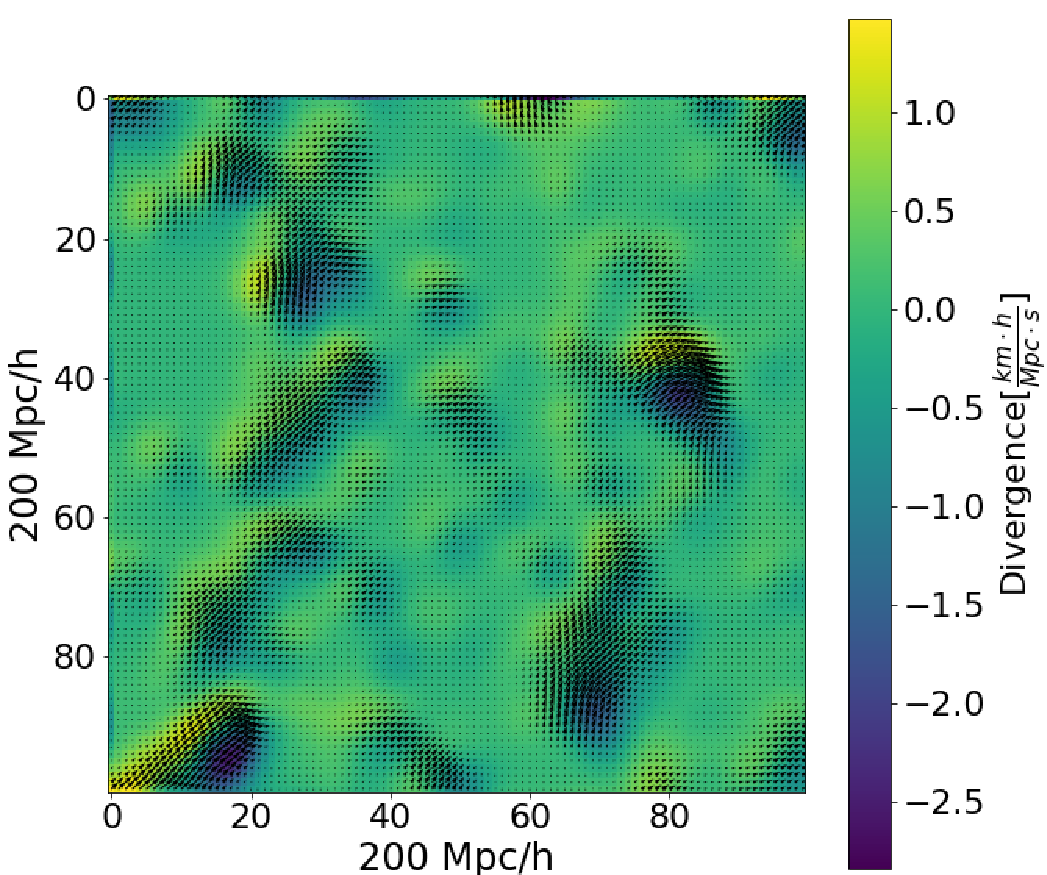
\includegraphics[width=240pt]{grad_vel_fields.pdf}
    \caption{In a cross section of the 3D grid at a random X, the corresponding  velocity vectors in Y and Z are shown in black. The divergence field is shown in colors, where yellow zones have a big positive divergence and dark blue regions are those with big negative values for it. Notice how in these structures the divergence is much more negative in the center of the agglomerations than in the rest of the structure and how the whole structure has bigger velocity vectors than the remain regions.}
    \label{fig:grad_vel_fields}
\end{figure}



\subsection{Watershed algorithm}
 Hence, in order to define geometric boundaries for random objects a powerful tool called  the \textbf{Watershed Algorithm} is used. For this problem the watershed method is fundamental for the recognition of clusters and, therefore, it is the backbone of this work. The algorithm assigns an integer as the identifier for each voxel evaluated. This integer is in ascending order, for simplicity of the algorithm. For example, the identifier \texttt{'1'} was assigned to the group associated with the \texttt{first} seed that was found, the identifier \texttt{'255'} was assigned to the group of the \texttt{255th} seed and so on. 
 
 If the algorithm works properly, the regions that the algorithm segregates should be able to be compared at a glance with the perturbations of the divergence field. This can be seen in Figure \ref{fig:1Pert}, where a section of the smoothed divergence field with $\sigma_{Vox} = 1$ and its respective classification is shown. Figure \ref{fig:3Pert} shows the same cut of the grid, this time smoothed with $\sigma_{Vox} = 5$, where it is easy to notice that in this last case the regions found are larger, which also implies a lower number of regions found.
 
 As expected, the first groups that the algorithm recognizes are those whose origin had very high accretion. These high accretion centers belong to the largest superclusters, which are expected to have the lowest identifiers.

\begin{figure}
    \centering
    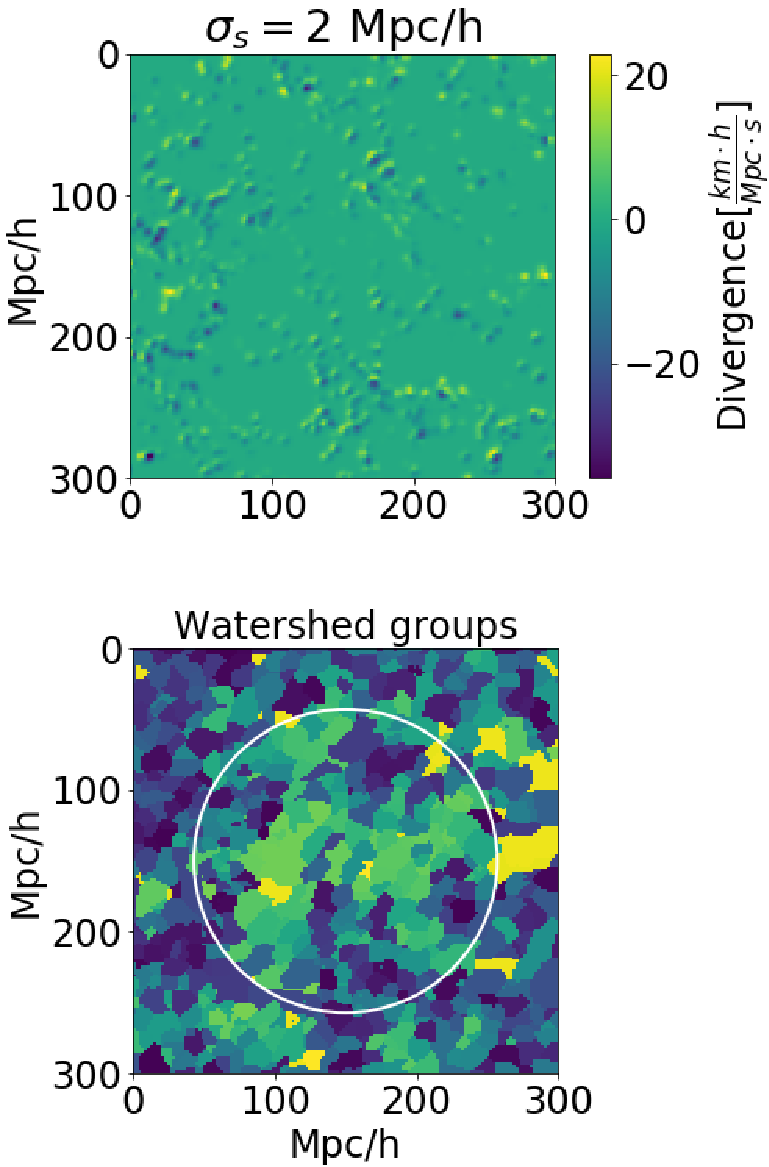
\includegraphics[width=220pt]{smooth_watershed_01.pdf}
    \caption{On the left there is a random cut on the axis where the regions with different accretion are observed. On the right the classification made by the Watershed method is shown, where different regions have different colors. Both figures were made using a smoothing scale of $\sigma_{Vox}$ = 1. Notice how a large number of superclusters are found by the algorithm and the correspondent absent of structures in the divergence figure.}
    \label{fig:1Pert}
\end{figure}

\begin{figure}
    \centering
    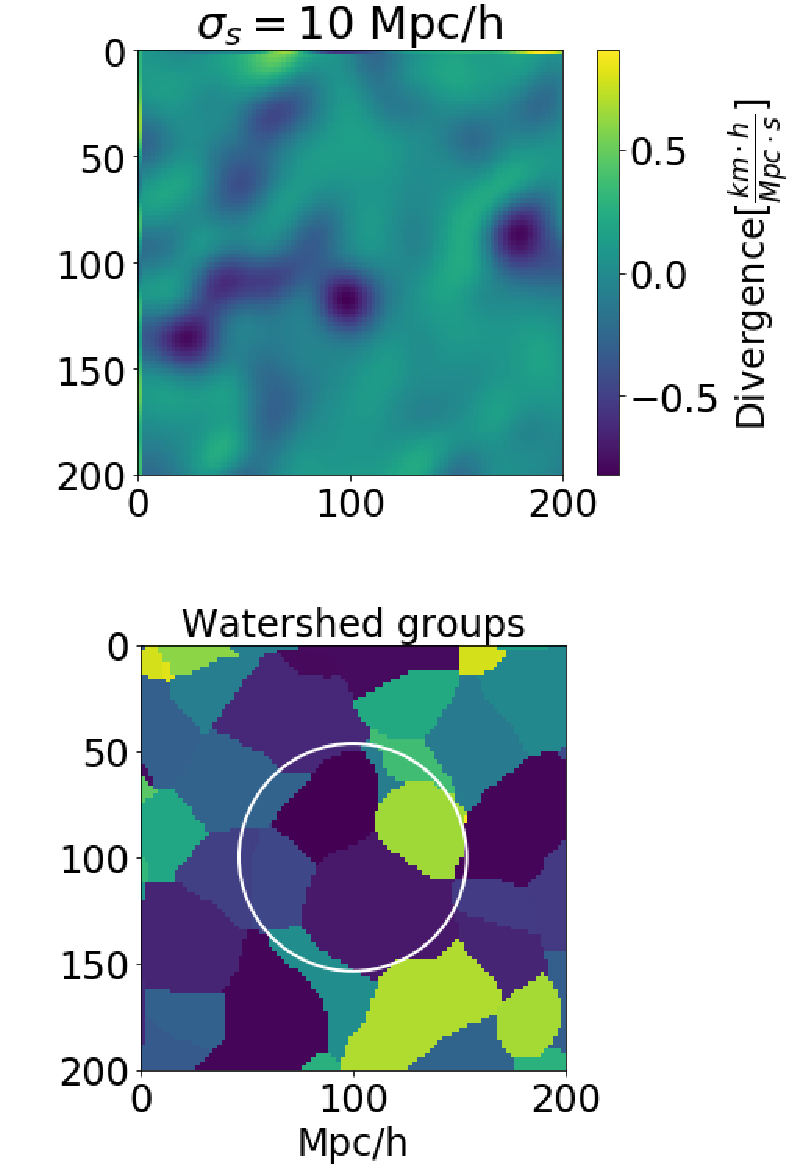
\includegraphics[width=220pt]{smooth_watershed_05.pdf}
    \caption{This graph shows the same cross section as Figure \ref{fig:1Pert}, but this time the field was smoothed with $\sigma_{Vox}$ = 5. In this case, a lower number of sperclusters is found in the same cut of the 3D grid. In both graphs it is seen how the distinguishable accretion peaks are classified as independent regions by the algorithm.}
    \label{fig:3Pert}
\end{figure}
As for the shape of the regions, superclusters are expected to have random and therefore unpredictable forms. However, it is possible to establish patterns that the regions must follow to determine if the algorithm is faulty or inefficient. For example, it is expected that in regions of void, i.e. those with negative accretion, the borders of many regions will be brought together. This is because they are the last parts of the scalar map that the surveyed of watershed evaluates. Figure \ref{fig:3Pert} shows a huge void where this predicate can be corroborated.


\subsubsection{Sigma Influence Analysis}
\label{sec:Sigmainfluence}
Watershed's algorithm was performed on the divergence grid built with smoothed speeds of the simulations with certain  $\sigma_{Vox}$. This method finds a determined number of superclusters in the entire space and assigns each supercluster a group identifier. If the method was used, it is worth saying that all the points in the grid already belong to a group.

\begin{figure*}
    \centering
    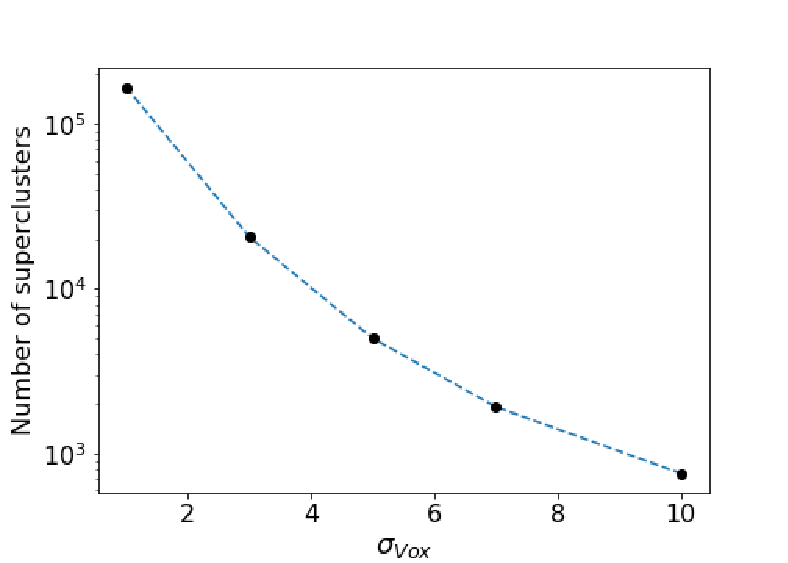
\includegraphics[width=240pt]{num_superclusters.pdf}
    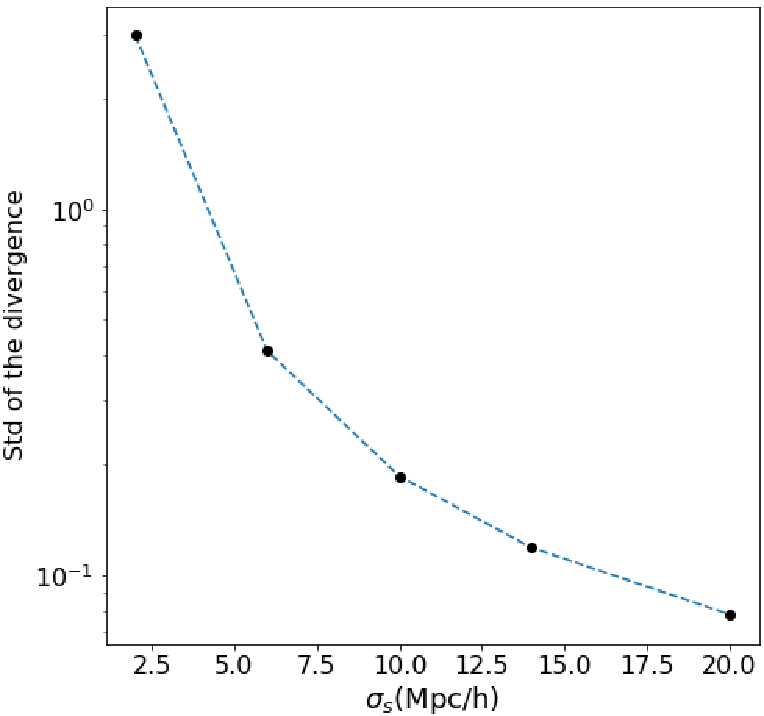
\includegraphics[width=240pt]{std_smooth.pdf}
    \caption{Behaviour of the number of superclusters found in a simulation and the standard deviation of the divergence field of the simulation as a function of the smoothing scale parameter $\sigma_{Vox}$. Effectively a smaller $\sigma_{Vox}$ implies recognizing many more structures; This is because each structure is of a smaller volume and a larger quantity is required to fill the entire space of the simulation. In addition, a smaller $\sigma_{Vox}$ implies that a lighter softened is been applied on the data and it produces a less smooth distributed grid.}
    \label{fig:Nclusters}
\end{figure*}

When defining different $\sigma_{Vox}$, it is expected that prominent fluctuations in the divergence field occupy a greater or lesser volume depending on the chosen $\sigma_{Vox}$. Similarly, it is expected that by using a larger $\sigma_{Vox}$, for example, the method classify superclusters that are larger and therefore a lower number of them will be found. Figure \ref{fig:Nclusters} shows the number of superclusters classified for each $\sigma_{Vox}$, as  well as the behaviour of the standard deviation of the divergence as a function of $\sigma_{Vox}$. In both plots it is observed that the $\sigma_{Vox}$ is indeed relevant in the definition of large scale strutures in simulations.


\subsection{Supercluster characterization}

As presumed, the borders of the grupus found by the algorithm are not smooth and it is a varied \emph{Zoo} of shapes and sizes. Now we have a catalog of superclusters in the simulation, with definite volumes in the grid and, therefore, with a mass that is also defined. In particular, the values of mass and volume of the structures found by the algoritm are expected to give us information about how the distribution of mass in space is being modified. Therefore, superclusters with larger mass and volume should have more mass coming together in it. As a result, bigger values of negative divergence have to be observed in these structures. This behaviour is presented in figure \ref{fig:min_div} where it is shown how higher mass and volume superclusters tend to have lower minimum values the divergence field, as expected from its definition of regions of converging galaxy flows. 


\begin{figure*}
    \centering
    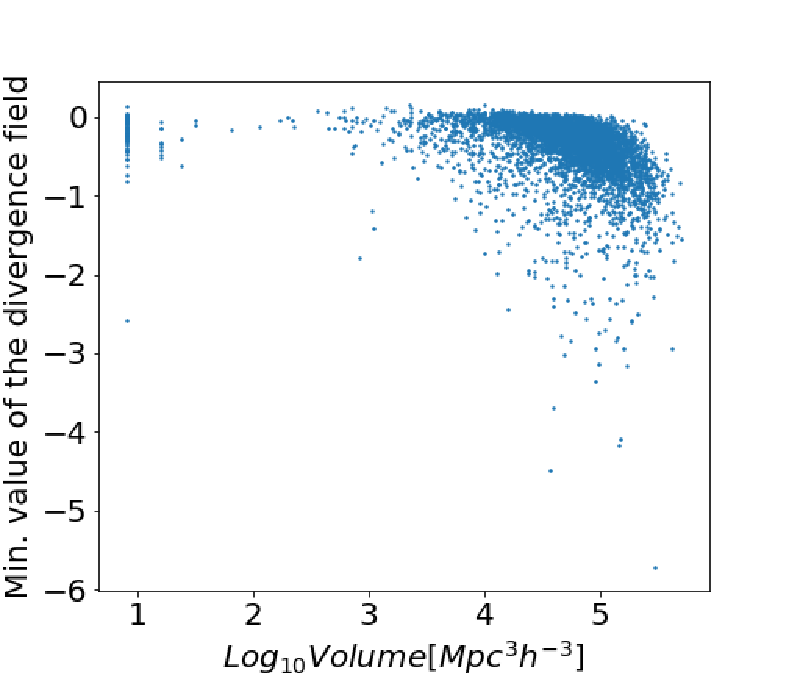
\includegraphics[width=240pt]{min_div_volume.pdf}
    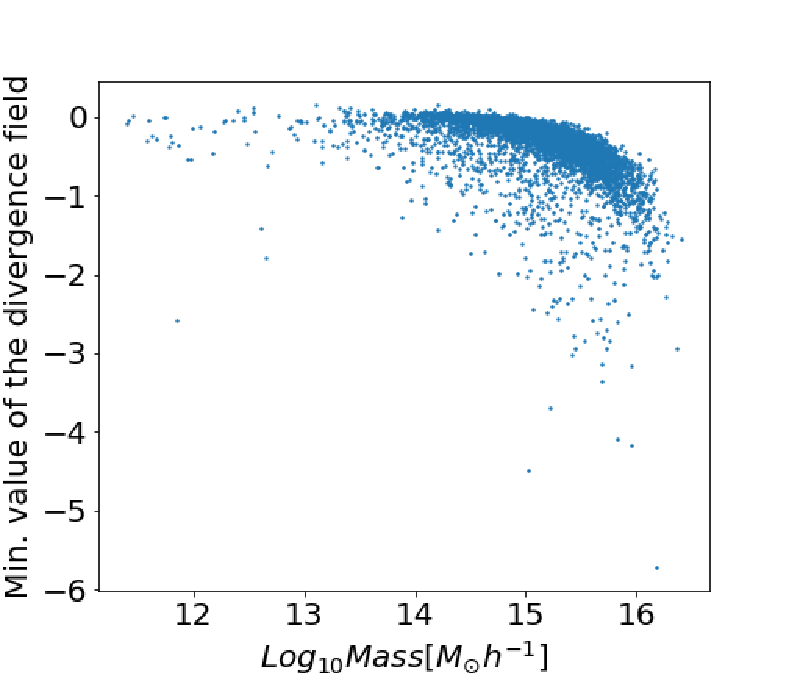
\includegraphics[width=240pt]{min_div_mass.pdf}
    \caption{Relation of the minimum value of the divergence field in a supercluster according to its mass and its volume. Both panels show that higher mass and volume superclusters tend to have lower minimum values the divergence field, as expected from its definition of regions of converging galaxy flows. This analysis was realised using a gaussian smoothing scale of $\sigma_{Vox}$ = 5 and a simulation which uses Planck 2015 parameters.}
    \label{fig:min_div}
\end{figure*}


Each voxel already belongs to a group as well as the mass it contains and it is easy to extract new information from mass and volume statistics. By extension, these data also allow conclusions to be drawn about density. In order to achieve this analysis correctly two different sets of simulations where considered. First, we consider a set of five simulations of the Abacus Cosmos 720box\_planck catalog. Second, we vary the values of the cosmological parameters used in the simulations to see how this affects to the mass, volume and density distributions of the superclusters found. Specifically, extreme values of $\Omega_M$ and $\sigma_8$ are taken since these parameters could cause a significant difference in the distributions of the desired magnitudes. In this way, the higher and lower values of $\Omega_M$ and $\sigma_8$ in the AbacusCosmos\_720box catalog are identified and the simulations associated to those values added to our data set. In addition, a reference simulation, which was taken from the Abacus Cosmos 720box\_planck catalog, is added to this data set.

\subsubsection{Mass, Volume and density}

The Gaussian smoothing process, as well as the watershed algorithm, are applied to the two data sets presented above.  Once we have the superclusters found by the algorithm for each simulation, a comparison between Laniakea and the superclusters identified can be made. Figures \ref{fig:HISTVMD1} and \ref{fig:HISTVMD2} show how normal is Laniakea when we contrast it with the set of simulated superclusters. 
Figure \ref{fig:HISTVMD1} presents the distributions of mass, volume and density for each simulation of the first data set (only planck parameters simulations) and the respective value for Laniakea of each one of these variables. An atypical behaviour is observed as Laniakea is at the edges of the distributions and in an atypical region of the density histogram. In particular, Laniakea is found to be much more large, massive and dense than most of the superclusters identified by the algoritm. In addition, figure \ref{fig:HISTVMD1} exhibit a mass vs volume diagram in which the atypical behaviour is observed, as our supercluster is found out of the central group of superclusters.

Figure \ref{fig:HISTVMD2} shows how a significant change on the values of $\Omega_M$ and $\sigma_8$ affects the distributions of mass, volume and density of the superclusters. A similar result as in figure \ref{fig:HISTVMD1} is observed as Laniakea is still at the edges of the density histograms. In other words, the rareness of Laniakea, with respect to the groups stablished by the watershed algoritm, is independent on the choice of the values of cosmological parameters. In particular, when varying $\Omega_M$ and $\sigma_8$.


\begin{figure*}
    \centering
    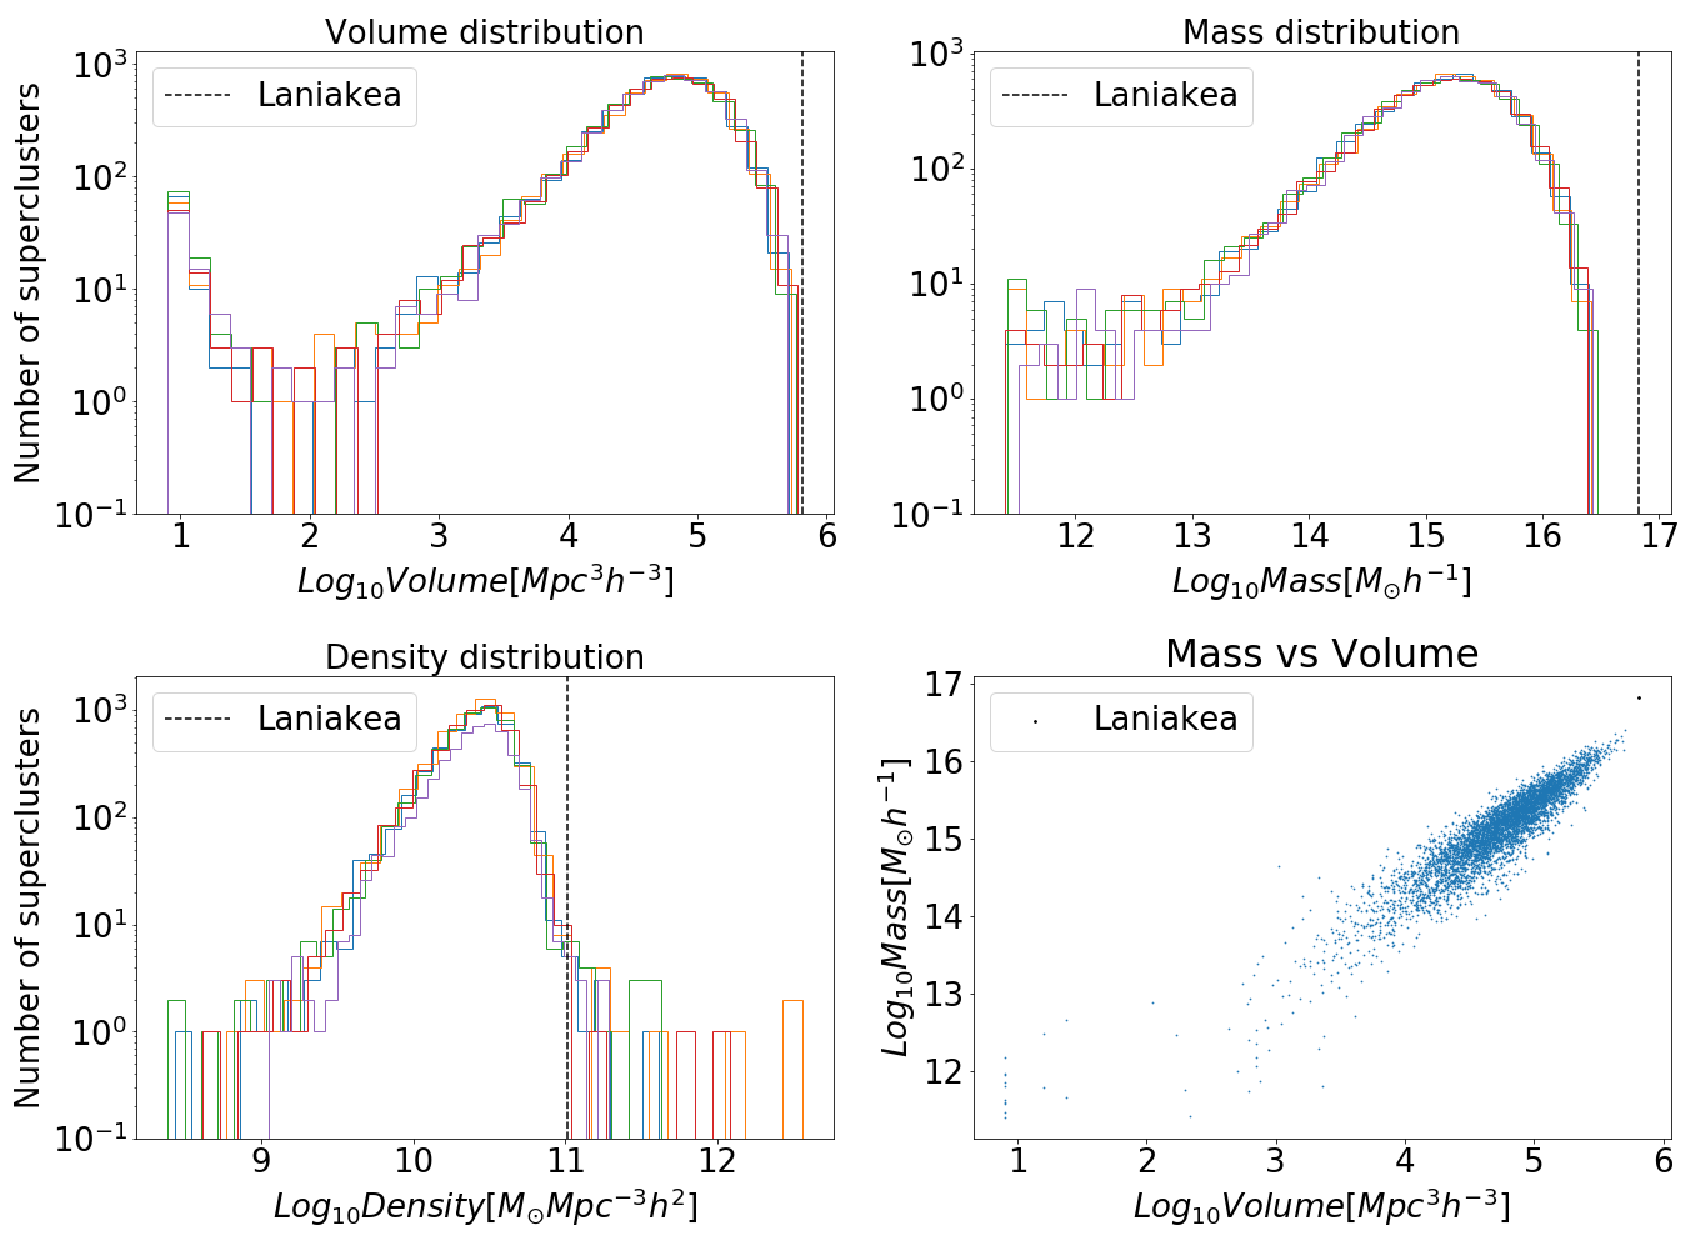
\includegraphics[width=435pt]{mass_vol_planck.pdf}
    \caption{Distributions of mass, volume and density for the superclusters found with $\sigma_{Vox} = 5$ using the first 5 Abacus Cosmos simulations with Planck parameters. A graph of mass vs volume in the first simulation of the Abacus Cosmos catalog is also shown. Notice how, Laniakea is at the edges of the distributions and in an atypical region of the density histogram. }
    \label{fig:HISTVMD1}
\end{figure*}


\begin{figure*}
    \centering
    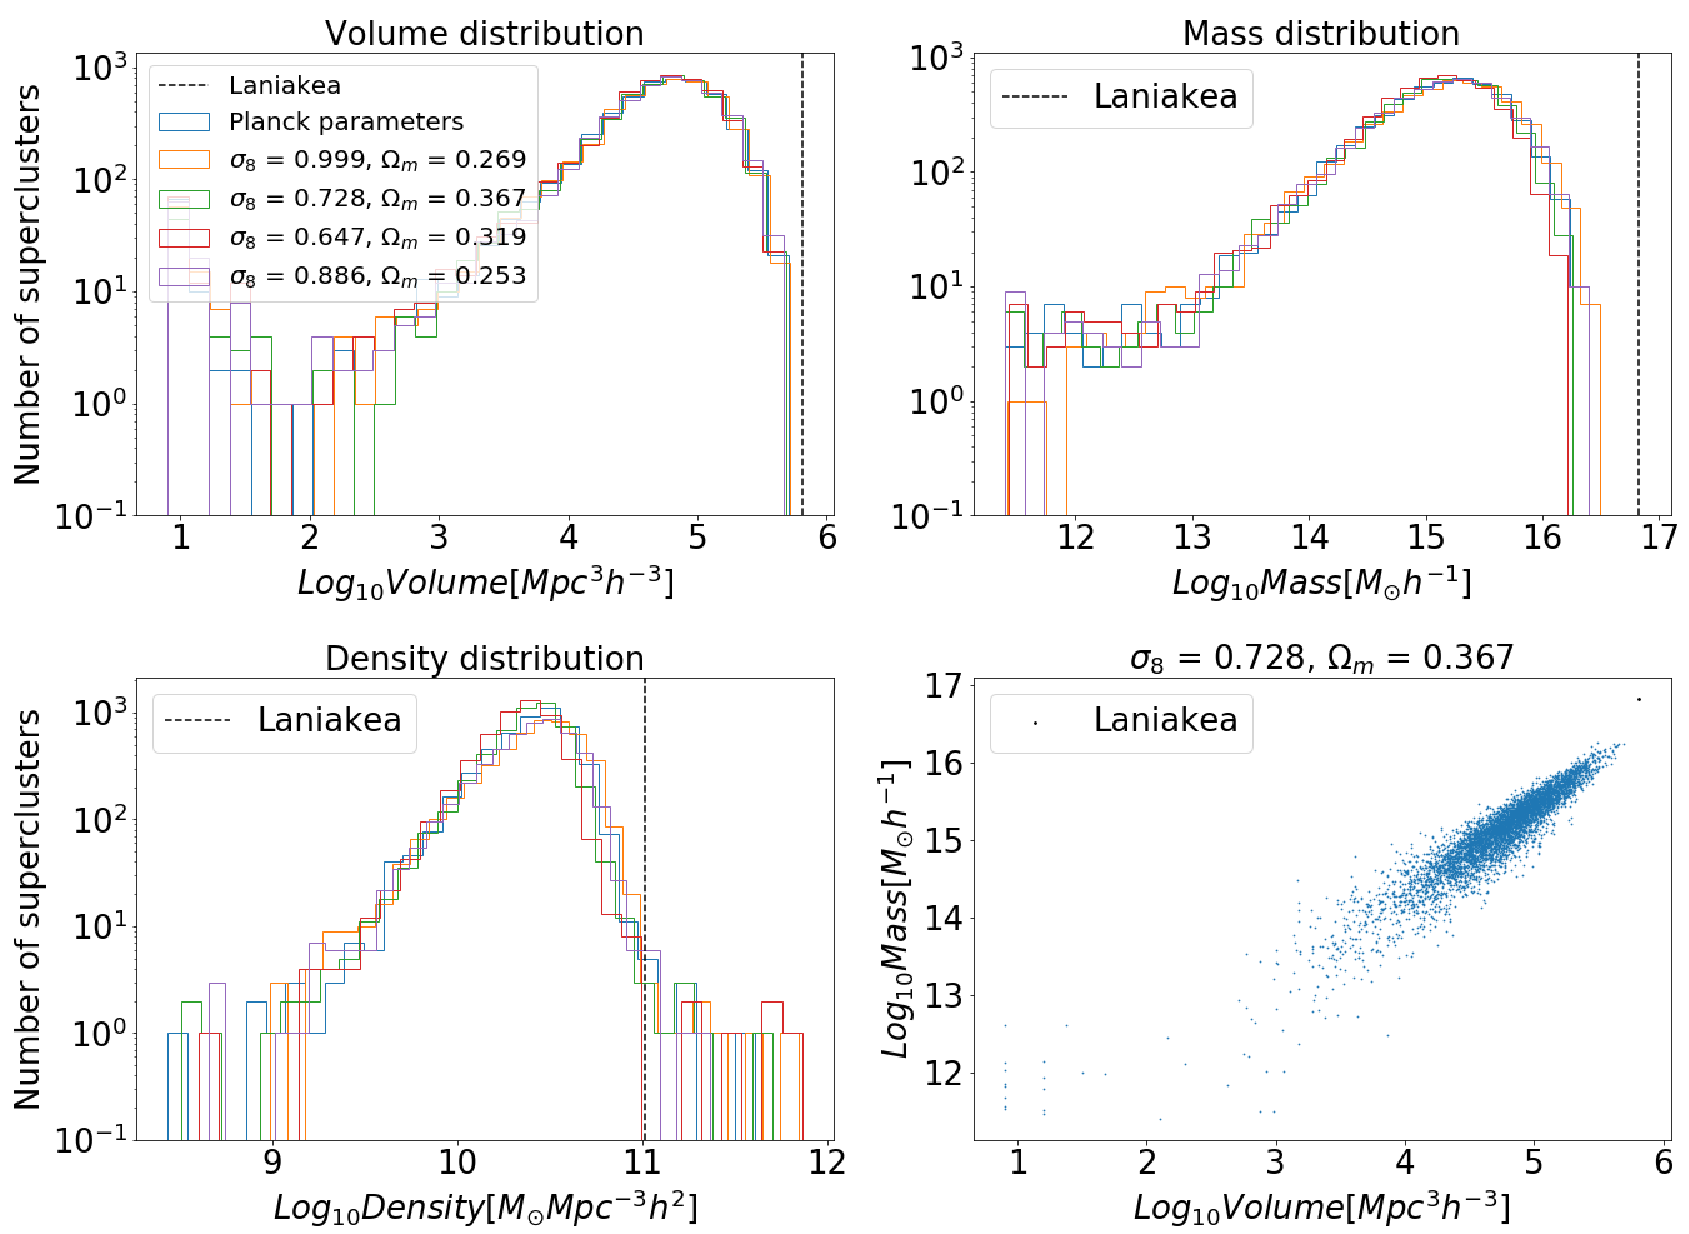
\includegraphics[width=435pt]{mass_vol_different.pdf}
    \caption{Distributions of mass, volume and density for the superclusters found with $\sigma_{Vox} = 5$ using the first Abacus Cosmos simulation with Planck parameters and the 4 simulations associated to extreme values of $\sigma_8$ and $\Omega_m$. A graph of mass vs volume in the first simulation of the Abacus Cosmos catalog is also shown. Notice how, Laniakea is at the edges of the distributions and in an atypical region of the density histogram. }
    \label{fig:HISTVMD2}
\end{figure*}



\section{Conclusions}
\label{sec:conclusions}

A recent result in this branch was the definition of our local supercluster Laniakea made by Tully el al.(2014)\cite{tully_laniakea_2014}, who used the velocity flow of galaxies for this purpose. Already having the characteristics of Laniakea, both in form and in mass, the next question would be how common it is among the other superclusters.

We divide the space of the simulation with a grid size close to the canonical length of \texttt{10 Mpc} used in observations to find Laniakea, which corresponds to a grid of [$120 \times 120 \times 120$].Once the velocity field is obtained, it is smoothed with Gaussian kernels of different width $\sigma_{Vox}$. Then the VDC is computed for each gridpoint. In order to differentiate structures from the order of the observable superclusters i.e. structures of about 10 Mpc $h^{-1}$, we use $\sigma_{Vox} = 1$ Vox. Using larger values of $\sigma_{Vox}$ does \texttt{NOT} yield erroneous information, but information with little usefulness about formation in a much larger scale.  

The implementation of the Watershed algorithm was a complete success. It managed to segregate regions based on the divergence field. Two parameters, $R_T$ and $Q_T$, are defined to control the algorithm and the segregation it makes. $R_T$ is of high relevance since it indirectly dictates the number of \emph{origins} that there are in the map and, therefore, the number of superclusters that will be in the space of the simulation. $Q_T$, on the other hand, does not affect the analysis carried out by the algorithm in a meaningful way since it rather indirectly defines the top of watershed sweeps that must be made before proceeding to classify the voxels by distance.

With the superclusters segregated and characterized we compare their propoerties against Laniakea. We find that our supercluster is  atypical according to its mass, volume and shape. On the other hand, the density of Laniakea seems to be frequent in the supercluster population since it is in a range close to the average. The populations with which Laniakea is compared within the simulation are small, either evaluating its mass, its volume or its shape. This makes it difficult to find a supercluster in the simulation that is similar to Laniakea within the ranges defined in Figures \ref{fig:HISTVMD1} and \ref{fig:INERTIA} at the same time. The probability of finding in the simulation a supercluster similar to Laniakea in those three aspects is a little lower than 0.07\%.

Regarding future work, we strongly suggest to experiment with the initial conditions of the problem and with the definition of the grid. A proposal is to define a grid with distances less than 10 Mpc $h^{-1}$, that is, with a higher value of $N_{side}$ and therefore with greater definition. You can also try different mass cuts for the Halos, different simulations of the same cosmology used in this work or even simulations in the context of different cosmologies.\\

\bibliographystyle{mnras}
\bibliography{references}



\end{document}
